\chapter[An introduction to Statistical Learning Theory]{An introduction to\\ Statistical Learning Theory}
\label{chap:intro}

\minitoc

\addchapterlof
\addchapterloa
\addchapterloe

\begin{abstract}
    This chapter provides an overview of statistical learning theory.
    We introduce the main concepts and notations used in this thesis focusing on supervised learning.
    Moreover, we review the main theoretical frameworks allowing one to derive some guarantees on the quality of the learning process.
\end{abstract}

\newpage

\section{Introduction}
\label{chap:intro:sec:intro}
Statistical learning encompasses a set of statistical methods that aims to automatically solve a task with the help of a computer from data.
For example, the task can consist in identifying a digit in an image.
In practice, the task is represented by a database (\aka dataset or learning sample) containing a finite number of examples.
More precisely, one example is composed of an input and its corresponding output (\aka label).
For the digit recognition problem, one example is made up of an image (the input) with its corresponding digit (the output).\\

To solve the task, we have to design a model that outputs the correct label given the input.
This model is usually a potentially complicated mathematical function.
From a human perspective, designing by hand a mathematical function that solves the task can be tedious.
Instead, in statistical learning, we aim to find {\it automatically} such a function with an algorithm.
This algorithm is usually called {\it learning algorithm} since the process of finding a function boils down to {\it learning} a function that solves the task.
The setting of statistical learning and the learning process is illustrated in \Cref{chap:intro:fig:intro}; it is defined more formally in the rest of the section.\\

\begin{figure}[H]
    \centering
    \includestandalone[width=0.8\textwidth]{chapter_1/figures/introduction}
    \caption[Representration of Statistical Learning]{
    \looseness=-1
    Rough representation of statistical learning for the digit recognition task. 
    On the left, each input (the handwritten digits) is represented in 2 dimensions.
    On the right, we illustrate the notion of learning, \ie, an algorithm finds a function (represented by the black line) predicting the digit 0 for the points belonging to the blue area and the digit 5 for those belonging to the white one.
    The black line is also called the decision boundary.
    }
    \label{chap:intro:fig:intro}
\end{figure}

\subsection{Representation of a Task}

\looseness=-1
This thesis studies the classification problem from a supervised learning perspective.
More formally, we consider a set of $d$-dimensional inputs $\X\subseteq \R^\d$ and a set of outputs $\Y$ (\aka set of labels).
In the binary classification setting, when $\Y=\{-1, +1\}$, the input is classified either into the label $-1$ or $+1$.
In the multi-class classification setting, when $\Y=\{1, 2, \dots, \L\}$, the input is classified into $\L\ge 2$ different labels.
Given an input set $\X$ and a label set $\Y$, we assume the task to be represented by an {\it unknown} function $\hbest: \X\to\Y$.
The unknown function $\hbest$ can be stochastic, meaning that $\hbest(\x)$ involves randomness, and thus different outputs $\y\in\Y$ are probable for the same input $\x\in\X$.
Moreover, some inputs $\x\in\X$ are more representative of the task, \ie, some inputs may be more probable than others.
To take this probabilities into account, the function $\hbest$ is replaced with an {\it unknown} distribution $\D$ on $\X{\times}\Y$; the distribution $\D$ represents the probability to sample a given input $\x\in\X$ and the output of the function $\hbest$.
More precisely, we assume that each couple $(\x, \y)\in \X{\times}\Y$ (\aka example) is a realization from this {\it unknown} data distribution $\D$ on the set $\X{\times}\Y$.
Even if the distribution $\D$ is {\it unknown}, we usually assume that we have access to some examples that we hope to be sufficiently representative and sampled from $\D$.
This set of examples is defined as follows.

\begin{definition}[Learning sample]
We define as {\it learning sample} (or {\it training set}) a set of $\m$ random variables {\it independent and identically distributed} (\iid) following the distribution $\D$.
We have
\begin{align*}
    &\S \defeq \bigcup_{i=1}^{\m}\Big\{ (\x_i, \y_i) \Big\}  \defeq \Big\{ (\x_i, \y_i) \Big\}_{i=1}^{\m}\subseteq (\X\times\Y)^\m,\\
    &\quad\text{where}\quad \forall i\in\{1,\dots,\m\},\quad (\x_i, \y_i){\sim}\D  \quad\text{and}\quad \S = \Big\{ (\x_i, \y_i) \Big\}_{i=1}^{\m} \sim\D^{\m}
\end{align*}
The notation $\D^\m$ denotes the distribution of $\m$ examples following $\D$: 
\begin{align*}
    \D^\m\big(\{ (\x_i, \y_i)\}_{i=1}^{\m}\big) = \D^\m\big(\S\big) \defeq \prod_{i=1}^\m\D\big((\x_i, \y_i)\big).
\end{align*}
\end{definition}

\looseness=-1
In practice, the set of examples, organized in a dataset, can be created manually by a human and/or collected automatically by a computer.
One famous dataset associated with the digit recognition task is the MNIST dataset from~\citet{LeCunCortesBurges1998}.
For instance, the set of inputs $\X$ is the set of gray-scale images of size $28{\times}28$, and the set of labels $\Y=\{0, \dots, 9\}$ is the set of possible digits.
The learning sample $\S$ is composed of $m=60{,}000$ pairs of images (input) and digit (label).
A schematic representation of this task is presented in \Cref{chap:intro:fig:distribution}.

\begin{figure}[H]
    \centering
    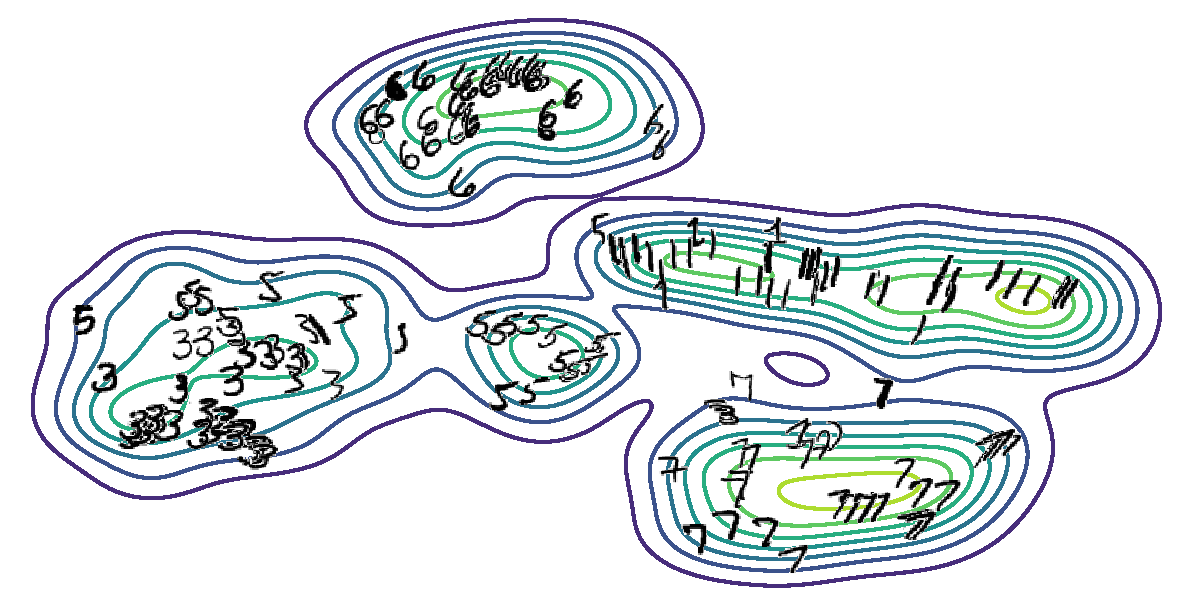
\includegraphics[width=\textwidth]{chapter_1/figures/distribution.pdf}
    \caption[Schematic Representation of a Data Distribution]{Schematic representation of the distribution $\D$ for the digit recognition task.
    The density of the distribution $\D$ is schematized with the contour lines where the purple \resp green is a low \resp high-density region.
    The examples (\ie, the handwritten digits) are sampled in high-density areas.
    A subset of the learning sample $\S\sim\D^\m$ is represented.}
    \label{chap:intro:fig:distribution}
\end{figure}


Deducing a mathematical model that predicts, for all $i\in\{1,\dots,\m\}$, the output $\y_i$ for the input $\x_i$ is not necessarily trivial.
To overcome this problem, statistical learning methods are developed to find {\it automatically} such a model that aims to solve the task by predicting the examples $(\x_i, \y_i)\in\X\times\Y$ correctly.

\subsection{``Solving'' a Task}

The model found automatically by the statistical learning method is actually a function $\h:\X\to\Y$ (called hypothesis in statistical learning theory) that takes an input $\x\in\X$ and outputs $\h(\x)\in\Y$.
This hypothesis $\h$ is selected by a learning algorithm among different candidates in a {\it  hypothesis set} $\H$ potentially infinite.
As an illustration, we recall four types of hypotheses used in practice.

\subsubsection{Examples of Hypotheses}

The four types of hypotheses we recall are the decision stump~\citep{IbaLangley1992}, the decision tree~\citep{BreimanFriedmanOlshenStone1984}, the linear classifier, and the neural network.
More precisely, these hypotheses are called {\it classifier} since they classify an input $\x\in\X$, \ie, assign a label to an input. 

\paragraph{Decision Stump}

The decision stump~\citep{IbaLangley1992} is a classifier composed of one decision rule of the form ``Is $x_i \le \threshold$?'', where $x_i$ is the $i$-th component of the vector $\xbf$ and $\threshold\in\Rbb$ is a threshold.
More precisely, this {\it decision rule} (implemented as an if-condition) assigns a label to the input $\x$.
For example, we present in \Cref{chap:intro:algo:stump} a decision stump that classifies the input $\x$ as $+1$ when $x_1 \le 0.54$ and $-1$ otherwise.
Its graphical representation and the associated decision are given in \Cref{chap:intro:fig:stump}.

\begin{algorithm}[H]
 \caption{Example of Decision Stump}
  \begin{algorithmic}
  \State{{\bf Given: } An input $\x\in\R^\d$}
    \If{$x_1 \le 0.54$}
        \State{\Return{$+1$}}
    \Else
        \State{\Return{$-1$}}
    \EndIf
  \end{algorithmic}
  \label{chap:intro:algo:stump}
\end{algorithm}

\begin{figure}[H]
    \centering
    \includestandalone[width=0.8\textwidth]{chapter_1/figures/decision_stump}
    \caption[Example of Decision Stump]{Example of decision stump with the decision rule ``Is $x_1 \le 0.54$?''.
    On the left, the decision of \Cref{chap:intro:algo:stump} is shown with its binary tree representation.
    The right plot shows the decision boundary (in white and blue) of the given decision stump.
    Moreover, the red triangles \resp the blue dots are the examples in the learning sample $\S$ with the label $+1$ \resp $-1$. 
    }
    \label{chap:intro:fig:stump}
\end{figure}

To classify the input $\x\in\X$, the decision stump returns a label (by executing its associated algorithm). 
This algorithm is composed of only one if-condition that can be interpreted as a binary tree.
This simple classifier can be complexified by adding more if-conditions to fit the data better.
Indeed, a decision tree can be constructed by considering nested if-conditions.
Hence, the decision stump\footnote{\citet{IbaLangley1992} introduced the word ``stump'' for a one-level decision tree.} is a particular case of a decision tree~\citep{BreimanFriedmanOlshenStone1984}.

\paragraph{Decision Trees}

The {\it decision tree}~\citep{BreimanFriedmanOlshenStone1984} is a classifier that can be seen as a succession of {\it decision rules} to classify the label of the input $\x\in\R^\d$.
\Cref{chap:mv:algo:decision-tree} is an example of algorithm associated to the decision tree of \Cref{chap:mv:fig:tree}.
 
\begin{figure}[H]
    \centering
\begin{algorithm}[H]
 \caption{Example of Decision Tree}
  \begin{algorithmic}
  \State{{\bf Given: } An input $\x\in\R^\d$}
    \If{$x_1 \le 0.59$}
        \If{$x_2 \le 0.63$}
            \State{\Return{$+1$}}
        \Else
            \State{\Return{$-1$}}
        \EndIf
    \Else
        \State{\Return{$-1$}}
    \EndIf
  \end{algorithmic}
  \label{chap:mv:algo:decision-tree}
\end{algorithm}
    \includestandalone[width=0.8\textwidth]{chapter_1/figures/tree}
    \caption[Example of Decision Tree]{Example of decision tree composed of two decision rules ``Is $x_1\le 0.59$?'' and ``Is $x_2\le 0.63$?''.
    The binary tree on the left is the graphical representation of the decision stump.
    The right plot is the stump's decision boundary on the 2-dimensional data in $\S$ (with the red triangles and the blue dots).}
    \label{chap:mv:fig:tree}
\end{figure}

Numerous algorithms have been developed to infer decision trees \citep[see \eg,][]{BreimanFriedmanOlshenStone1984,Quinlan1986,Quinlan1993}.
One of the most popular is the CART algorithm~\citep{BreimanFriedmanOlshenStone1984}: it is, \eg, implemented in the well-known library \sklearn~\citep{Pedregosa2011}.
This algorithm is summarized as follows. 
The algorithm tests the decision rules ``Is $x_i \le \threshold$?'' with different components $x_i$ and thresholds $\threshold$.
Given a new decision rule, the examples $(\x,\y)\in\S$ are split into two groups: the ones that respect the rules and those that do not.
Then, the algorithm selects the best decision rule according to a criterion and the two new groups.
Finally, this step is repeated recursively to obtain the entire tree.
In \Cref{part:contrib-pac-bayes}, we learn a {\it majority vote} classifier which is a convex combination of the outputs of decision trees or decision stumps.

\paragraph{Linear classifier} One of the most simple type of classifiers is the linear classifier. 
Given a function $\act: \Rbb \to \Rbb$, this type of classifier is defined as 
\begin{align*}
    \h(\x) = \act\!\LP \sum_{i=1}^{\d}w_ix_i+\bias\RP,
\end{align*}
where $\w\in\Rbb^\d$ is the weight vector and $\bias\in\Rbb$ is the bias that both need to be learned.
The function $\act()$ is called {\it activation} function notably in the context of neural networks (that we precise in the following). 
For instance, the Perceptron~\citep{McCullochPitts1943,Rosenblatt1958} algorithm returns a linear classifier with the activation function $\act()$ called threshold function defined as $\act(x)=1$ if $x\ge 0$ and $\act(x)=0$ otherwise.
Moreover, the well-known Support Vector Machine (SVM) algorithm introduced by \citet{BoserGuyonVapnik1992,CortesVapnik1995} learns a linear classifier with the sign as activation function, \ie, $\act(x) = \sign(x)=+1$ if $a\ge 1$ and $-1$ otherwise.
We provide two 2-dimensional cases when the activation function is the sign function in \Cref{chap:intro:fig:linear}.

\paragraph{Neural networks.} 

\begin{figure}
    \centering
    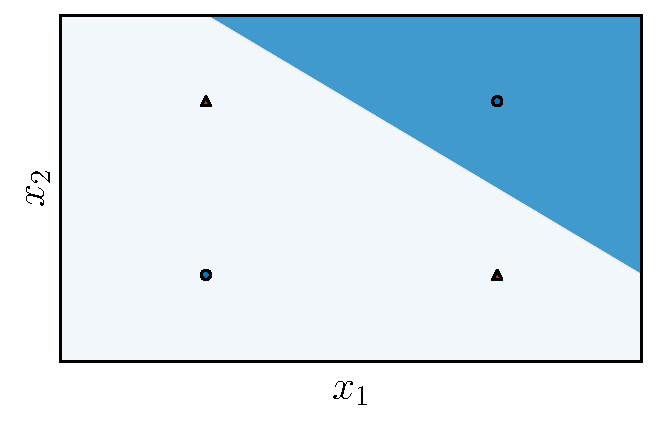
\includegraphics[width=0.8\textwidth]{chapter_1/figures/xor.pdf}
    \caption[Plot of the Exclusive Or Function]{
    Plot of the decision boundary of a linear classifier learned on the learning sample $\S{=}\{([0, 0]^\top, -1), ([0, 1]^\top, +1), ([1, 1]^\top, -1), ([1, 0]^\top, +1)\}$ that  represents the exclusive or function. 
    As proved by \citet{MinskyPapert1972}, this model cannot predict correctly all the examples representing such a function.
    }
    \label{chap:intro:fig:xor}
\end{figure}

The Perceptron was abandoned when \citet{MinskyPapert1972} show that this model cannot learn simple (boolean) functions like the exclusive or (see \Cref{chap:intro:fig:xor}).
Hopefully, these restrictions are avoided when generalizing the Perceptron, and they regain interest in the 80s.
Nevertheless, in the 2010s, these models have become popular when the neural network AlexNet~\citep{KrizhevskySutskeverHinton2012} won the computer vision challenge ``ImageNet Large Scale Visual Recognition Challenge''.
The increase in popularity of such models has been helped by the existence of many programming frameworks such as \torch~\citep{CollobertKavukcuogluFarabet2011}, \tensorflow~\citep{Abadi2015}, \theano~\citep{AlRfou2016}, \jax~\citep{FrostigJohnsonLeary2018,Bradbury2018}, or \pytorch~\citep{Paszke2019}.
To learn more details about neural networks, we refer the reader to \citet{GoodfellowBengioCourville2016} for an extensive introduction.
Actually, a neural network can be seen as a succession of linear classifiers: it is a composition of $L$ linear classifiers $\hvec^{(1)}(),\dots, \hvec^{(L)}()$ called layer or module, \ie,
\begin{align*}
    \h = \hvec^{(L)}\circ\dots\circ\hvec^{(2)}\circ\hvec^{(1)},
\end{align*}
where $f\circ g$ is the composition of the function $f()$ with $g()$.
More precisely, given an activation function $\actvec^{(i)}: \Rbb^{\d^{(i)}} \to \Rbb^{\d^{(i)}}$, the $i$-th layer $\hvec^{(i)}: \Rbb^{\d^{(i-1)}} \to \Rbb^{\d^{(i)}}$ of the network is defined by
\begin{align*}
    \hvec^{(i)}(\x) = \actvec^{(i)}\LP \wmat\x + \biasvec \RP,
\end{align*}
where the matrix $\wmat\in\Rbb^{\d^{(i)}\times\d^{(i-1)}}$ and the vector $\biasvec \in \Rbb^{\d^{(i)}}$ are respectively the weights and the bias parameterizing the classifier that need to be learned.
Note that, to respect the definition of the hypothesis $\h:\Rbb^\d\to \R$, we have $\d^{(0)}=\d$ and $\d^{(L)}=1$.

\begin{figure}
    \centering
    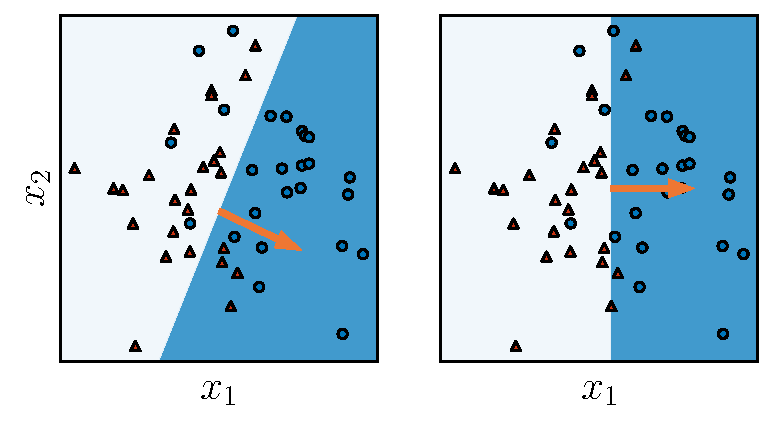
\includegraphics[width=0.8\textwidth]{chapter_1/figures/linear_classifier.pdf}
    \caption[Examples of Linear Classifiers]{
    The decision of two linear classifiers when the activation function is the $\sign$. 
    On the left plot, the weights are $\wbf=\LB3.2, -1.4\RB^\transp$ and the bias is $\bias=-1$.
    On the right plot, the weights are $\wbf=\LB1, 0\RB^\transp$ and the bias is $\bias=-0.54$; this linear classifier is equivalent to the decision stump in \Cref{chap:intro:fig:stump}.
    }
    \label{chap:intro:fig:linear}
\end{figure}

\begin{figure}
    \centering
    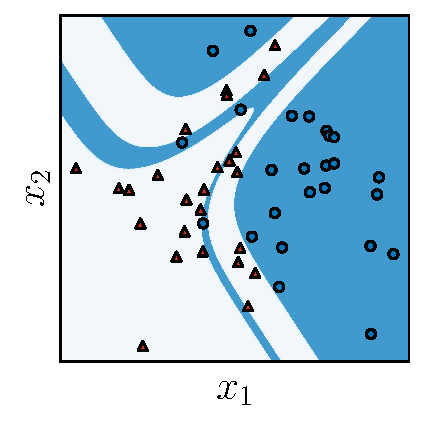
\includegraphics[width=0.5\textwidth]{chapter_1/figures/neural_network.pdf}
    \caption[Example of Neural Network]{
    The decision boundary of a neural network classifier of a with 5 layers and the dimensions $\d^{(1)}{=}\d^{(2)}{=}\d^{(3)}{=}\d^{(4)}{=}2$ and $\d^{(5)}{=}1$.
    The activation functions $\actvec^{(1)}(),\actvec^{(2)}(),\actvec^{(3)}(),\actvec^{(4)}()$ are $\tanh$ applied element-wise and $\actvec^{(5)}()$ is the threshold function. 
    }
    \label{chap:intro:fig:neural-network}
\end{figure}

\begin{figure}
    \centering
    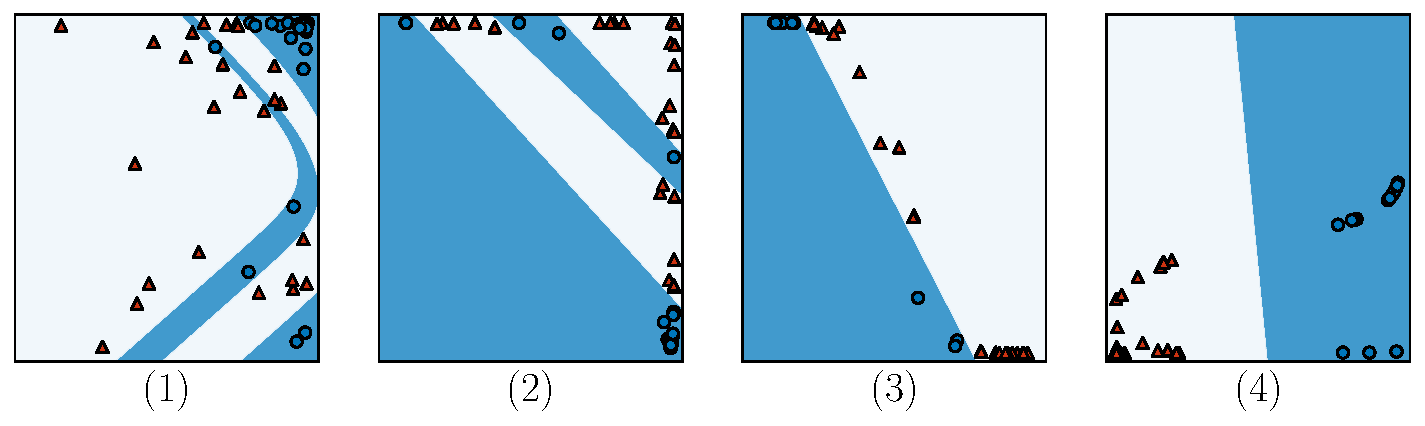
\includegraphics[width=1.0\textwidth]{chapter_1/figures/neural_network_full.pdf}
    \caption[Details on the Neural Network of \Cref{chap:intro:fig:neural-network}]{
    Each plot corresponds to the representation of the $i$-layer (where $i=1$ on the left plot and $i=4$ on the right plot).
    On each plot, the original examples $(\x,\y)\in\S$ (with the red triangles and the blue dots) are transformed and plotted by the $i$-th layer $(\hvec^{(1)}\circ\dots\circ\hvec^{(i)})(\x)$.
    Moreover, the decision boundary of the classifier $\hvec^{(i)}\circ\dots\circ\hvec^{(L)}$ is given.
    }
    \label{chap:intro:fig:neural-network-details}
\end{figure}

\looseness=-1
An example of neural network is given in \Cref{chap:intro:fig:neural-network}.
We see in this example that the succession of linear classifiers offers better expressiveness, \ie, its decision boundary is not restricted to lines.
Interestingly, these models produce new features of the original data in each layer.
Indeed, in \Cref{chap:intro:fig:neural-network-details}, the $i$-th layer transforms all inputs $\x\in\X$ into $\hvec^{(i)}(\dots\hvec^{(1)}(\x))$ and these new inputs are classified with $\hvec^{(L)}(\dots\hvec^{(i)}(\x))$.
Hence, all these transformations can be interpreted as a new representation of these inputs.
In the following, we denote by $\wbf\in\Rbb^D$ the vector of the network's weights and biases concatenated all together; we have thus $D$ weights/bias in the networks.
Besides, when $D$ is large compared to the number of data $\m$, we say in this case that the model is over-parametrized, and when $L$ is large, we consider that the network is ``deep''\footnote{The term deep learning comes from the fact that the number of layers $L$ is large.}.
This model is studied in \Cref{part:contrib-disintegrated} when the neural network is over-parametrized and ``deep''.

\subsubsection{Loss and Risk}
\label{chap:intro:sec:loss-risk}

We need to assess to which extent the learned hypothesis $\h\in\H$ predicts correctly an example. 
This kind of measure is often called a {\it loss function}, defined as follows.

\begin{definition}[Loss function]
A {\it loss} function is a function $\loss: \H\times (\X{\times}\Y) \to [0, 1]$ that, given a hypothesis $\h\in\H$, evaluates the quality of the prediction $\h(\x)$ compared to the true label $\y\in\Y$.
The lower the loss, the better the quality of the hypothesis.
\end{definition}

For a classification task, the most natural loss function is the 01-loss defined by
\begin{align*}
    \forall \h\in\H, \quad \forall(\x,\y)\in\X{\times}\Y,\quad \lossZO(\h, (\x,\y)) =\indic[\h(\x)\ne \y] \defeq \LC\begin{array}{cc}
        1 & \text{if}\  \h(\x) \ne \y\\
        0 & \text{otherwise}
    \end{array} \RE.
\end{align*}

The 01-loss returns $1$ when the hypothesis $\h\in\H$ misclassifies the example $(\x,\y)\in\X{\times}\Y$ and $0$ otherwise.
However, since many learning methods are based on the gradient $\frac{\partial\loss}{\partial\h}(\h ,(\x,\y))$ to choose a hypothesis $\h$ that lowers the loss function, the 01-loss $\lossZO()$ is not practical.
Its gradient $\frac{\partial\lossZO}{\partial\h}(\h ,(\x,\y))=0$ for all examples $(\x,\y)\in\X\times\Y$, which does not indicate a descent direction (that lowers the loss).
To address this issue, in practice, one uses relaxation of the 01-loss.
In particular, some relaxed losses rely on a notion of {\it margin}: in binary classification the margin is defined as $\Mah(\x,\y)=\y\h(\x)$ for all $h:\X\to[-1,+1]$.
When the margin is positive, the hypothesis makes a correct prediction.
In other words, the margin is defined such that we have $\lossZO(\h, (\x,\y))=\indic[\h(\x)\ne \y]=\indic[\Mah(\x,\y) \le 0]$.
Thanks to the margin and \textsc{Markov}'s inequality (\Cref{ap:tools:theorem:first-markov,ap:tools:theorem:snd-markov}), one can prove two upper bounds of the $01$-loss.
These two upper bounds are defined by
\begin{align*}
    &\lossFirst(\h, (\x,\y)) = 1-\Mah(\x,\y)\quad\quad \text{\citep{LangfordShaweTaylor2002}},\\
    \text{and}\quad &\lossSnd(\h, (\x,\y)) = \Big[1{-}\Mah(\x,\y)\Big]^2\quad \text{\citep{MasegosaLorenzenIgelSeldin2020}}.
\end{align*}
We plot in \Cref{chap:intro:fig:loss} the 01-loss and the two upper bounds that we use in \Cref{chap:mv-robustness,chap:mv} to derive learning algorithms.
We introduce these upper bounds with more details in \Cref{chap:pac-bayes}.

\begin{figure}[H]
    \centering
    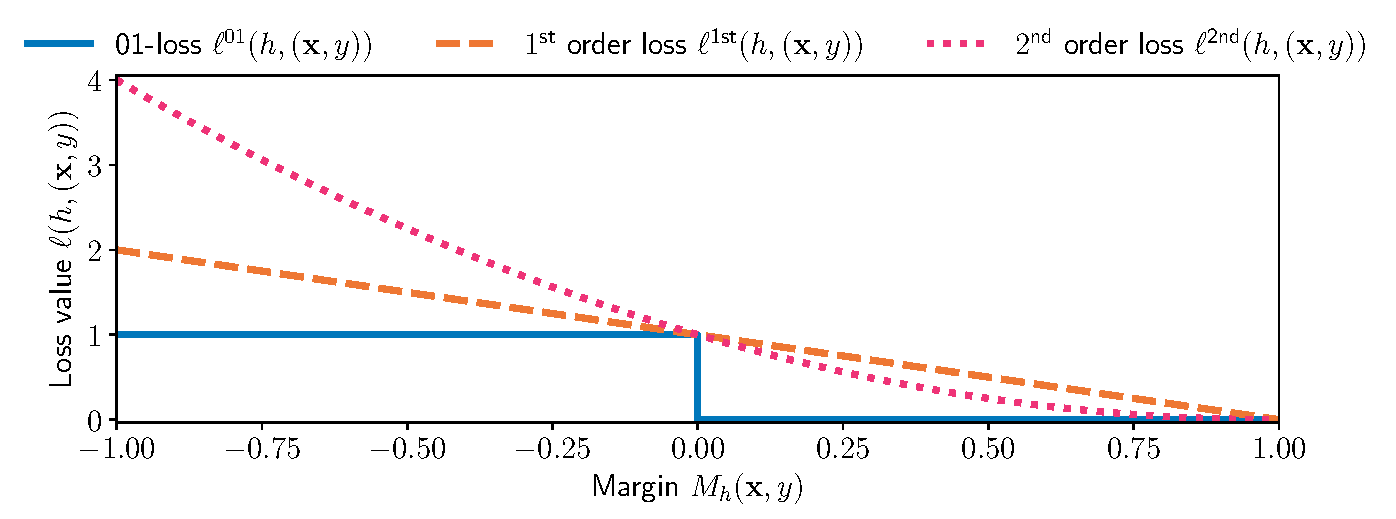
\includegraphics[width=1.0\textwidth]{chapter_1/figures/losses.pdf}
    \caption[Plot of Different Losses]{Plot of the losses ($\lossZO()$, $\lossFirst()$, and $\lossSnd()$) where the x-axis represents the value of the margin $\Mah(\x, \y)$ and the y-axis represents the value of the losses $\loss(\h, (\x,\y))$ for a given example $(\x,\y)$ and hypothesis $\h$.}
    \label{chap:intro:fig:loss}
\end{figure}

While the loss $\loss(\h, (\x,\y))$ is computed for an example $(\x,\y)$ and a hypothesis $\h$, we are usually interested in the loss computed over all the examples $(\x,\y)\in\S$.
The value of the loss averaged over the learning sample $\S$ is called {\it empirical risk} and represents to what extent the hypothesis $\h$ predicts correctly all the examples $(\x,\y)\in\S$.
The empirical risk is defined as follows.

\begin{definition}[Empirical Risk]
For any distribution $\D$ on $\X{\times}\Y$, for any learning sample $\S=\{(\x_i, \y_i)\}_{i=1}^{\m}\sim\D^{\m}$, we define the empirical risk as
\begin{align*}
    \RiskLoss_{\dS}(\h) \defeq \EE_{(\x,\y)\sim\dS}\loss(\h, (\x,\y)) = \frac{1}{\m}\sum_{i=1}^{\m}\loss(\h, (\x_i,\y_i)),
\end{align*}
where its associated uniform distribution $\dS$ on $\S$ can be defined as $\dS((\x_i,\y_i))\defeq\frac{1}{\m}$ for all $i\in\{1,\dots, \m\}$.
Moreover, we define the empirical risk with the 01-loss by
\begin{align*}
    \Risk_{\dS}(\h) \defeq \RiskLossZO_{\dS}(\h) = \frac{1}{\m}\sum_{i=1}^{\m}\indic\LB \h(\x_i) \ne \y_i\RB.
\end{align*}
\end{definition}

Since the distribution $\D$ is unknown, the performance of the hypothesis $\h\in\H$ can be computed by means of the learning sample $\S$ (through the empirical risk).
However, we are interested in the performance of $\h$ on the task, \ie, over all the examples.
The performance is thus defined through the true risk $\RiskLoss_{\D}(\h)$ defined as follows.

\begin{definition}[True Risk]
For any distribution $\D$ on $\X{\times}\Y$, for any loss function $\loss: \H\times (\X{\times}\Y) \to [0, 1]$, we define the true risk as
\begin{align*}
    \RiskLoss_{\D}(\h) \defeq \EE_{(\x,\y)\sim\D}\loss(\h, (\x,\y)).
\end{align*}
Moreover, we define the true risk with the 01-loss by
\begin{align*}
    \Risk_{\D}(\h) \defeq \RiskLossZO_{\D}(\h) = \EE_{(\x,\y)\sim\D}\indic\LB\h(\x) \ne \y\RB = \PP_{(\x,\y)\sim\D}\LB \h(\x) \ne \y\RB.
\end{align*}
\end{definition}

The true risk can be interpreted as the expected loss over all examples $(\x,\y)\sim\D$.
Actually, when the hypothesis $\h$ does not depend on $\S$, the true risk of $\h$ is the expected empirical risk.
In other words, the empirical risk can be seen as an unbiased estimator of the true risk, \ie, we have
\begin{align*}
    \EE_{\S\sim\D^\m}\RiskLoss_{\dS}(\h)=\EE_{\S\sim\D^\m}\frac{1}{\m}\sum_{i=1}^{\m}\loss(\h, (\x_i,\y_i))=\frac{1}{\m}\sum_{i=1}^{\m}\EE_{(\x_i,\y_i)\sim\D}\loss(\h, (\x_i,\y_i))=\RiskLoss_{\D}(\h).
\end{align*}

Besides, selecting a hypothesis with a low true risk boils down to finding a hypothesis with low empirical risk on average.
However, since we only have access to one learning sample $\S$, the hypothesis selection cannot be performed on the distribution $\D$ but rather on the learning sample $\S$.

\section{Hypothesis Selection}
\label{chap:intro:sec:selection}

In order to obtain a hypothesis $\h\in\H$ that solves the task, the hypothesis can be selected such that the empirical risk $\RiskLoss_{\dS}(\h)$ is low.
We recall two approaches from statistical learning: Empirical Risk Minimization (ERM) and Structural Risk Minimization (SRM). 

\subsection{Empirical Risk Minimization}

Given the hypothesis set $\H$, a common approach in statistical learning is to minimize the empirical risk $\RiskLoss_{\dS}(\h)$ with respect to the hypothesis $\h\in\H$. 
This approach -- known as {\it Empirical Risk Minimization} (ERM) -- has been pioneered by \citet{VapnikChervonenkis1968,VapnikChervonenkis1971,VapnikChervonenkis1974} in the 70s (see \citet{Vapnik1998} for an introduction).
Formally, given a learning sample $\S\sim\D^\m$, we select the hypothesis such that the empirical risk $\RiskLoss_{\dS}(\h)$ is minimum; this approach is summarized in \Cref{chap:intro:algo:erm}.

\begin{algorithm}[H]
  \caption{Empirical Risk Minimization}
  \begin{algorithmic}
    \State{{\bf Given:} Learning sample $\S$, Hypothesis set $\H$, Loss function $\loss: \H\times(\X{\times}\Y) \to [0,1]$}
    \State{\centerline{$\displaystyle\h = \argmin_{\h'\in\H}\RiskLoss_{\dS}(\h')$}}\\
    \Return{hypothesis $\h$}
\end{algorithmic}
\label{chap:intro:algo:erm}
\end{algorithm}

However, if the empirical risk $\RiskLoss_{\dS}(\h)$ of a hypothesis $\h\in\H$ is approximately $0$, then $\h$ potentially overfits the data; see~\Cref{chap:intro:fig:overfitting}.
Roughly speaking, in the case of overfitting, we interpret that $\h\in\H$ has learned by heart the examples in the learning sample.
Such a phenomenon can arise when the hypothesis $\h$ is complex; the complexity is manifested differently for each type of hypothesis.
To measure such complexity, a real-valued function can be defined $\comp: \H\times (\X{\times}\Y)^\m \to \Rbb$.
Given a learning sample $\S$ and a complexity function, the hypothesis $\h\in\H$ is considered complex when its associated complexity measure $\comp(\h, \S)$ is large.
In \Cref{chap:dis-mu}, we derive generalization bounds that integrate a user-specified complexity function.

\subsection{Structural Risk Minimization}

To avoid overfitting, we can select a hypothesis $\h$ with a small complexity measure $\comp(\h, \S)$. 
The {\it Structural Risk Minimization} approach -- introduced by \citet{VapnikChervonenkis1974} -- minimizes a trade-off between the empirical risk $\RiskLoss_{\dS}(\h)$ and the complexity measure $\comp(\h, \S)$.
The complexity measures $\comp()$ used in this approach is constant over the hypothesis $\h\in\H$ and the learning sample $\S\in(\X\times\Y)^\m$.
In other words, if we denote by abuse of notation $\comp(\H)$ the complexity measure associated to the hypothesis set $\H$, we have $\forall \h\in\H, \forall \S\in(\X\times\Y)^\m, \comp(\h,\S) = \comp(\H)$.
However, the complexity measure $\comp(\H)$ may not be representative of overfitting for a single hypothesis since $\comp(\H)$ is constant.
Hence, the hypothesis set $\H$ is structured into countable and nested hypothesis subsets $\H_1 \subseteq \H_2 \subseteq \dots \subseteq \H$.
By doing so, the complexity measure may be increasing when the hypothesis set grows: we can have $\comp(\H_i)\le\comp(\H_{i+1})$ when $\H_i\subseteq\H_{i+1}$. 
Then, thanks to these nested complexity measure, one can find a hypothesis $h$ belonging to a set $\H_i$ with $i\in\Nbb_*$ that minimizes the trade-off between the empirical risk $\RiskLoss_{\dS}(\h)$ and the complexity measure $\comp(\H_i)$ of the set $\H_i$. 
The minimization of the trade-off performed by the {\it Structural Risk Minimization} approach is summarized in \Cref{chap:intro:algo:srm}.

\begin{algorithm}[H]
  \caption{Structural Risk Minimization}
  \begin{algorithmic}
    \State{{\bf Given:} Learning sample $\dS$, Hypothesis set $\H$}
    \State{\centerline{$\displaystyle\h = \argmin_{i\in\Nbb_*,\  \h'\in\H_i}\LB \RiskLoss_{\dS}(\h') + \comp(\H_i) \RB$}}\\
    \Return{hypothesis $\h$}
\end{algorithmic}
\label{chap:intro:algo:srm}
\end{algorithm}

If the complexity measure $\comp(\H')$ of the subset $\H'\subseteq\H$ approximates well the difference $\RiskLoss_{\D}(\h)-\RiskLoss_{\dS}(\h)$, SRM can be used to obtain a hypothesis $\h\in\H'$ that {\it generalizes} well.
In other words, a hypothesis $\h\in\H'$ that {\it generalizes} has a small true risk $\RiskLoss_{\D}(\h)$ and empirical risk $\RiskLoss_{\dS}(\h)$ 
This situation is represented in \Cref{chap:intro:fig:overfitting}.
In other words, when $\h$ generalizes, the {\it generalization gap}\footnote{We consider sometimes the generalization gap  $\LN\RiskLoss_{\D}(\h)-\RiskLoss_{\dS}(\h)\RN$ instead, but, we are mostly interested in upper bounding the true risk $\RiskLoss_{\D}(\h)$.} $\RiskLoss_{\D}(\h)-\RiskLoss_{\dS}(\h)$ is close to $0$ (that is $\RiskLoss_{\D}(\h)\approx\RiskLoss_{\dS}(\h)$).
However, since the difference $\RiskLoss_{\D}(\h){-}\RiskLoss_{\dS}(\h)$ is not computable because of the true risk $\RiskLoss_{\D}(\h)$, we have to bound it.

\begin{figure}[H]
    \centering
    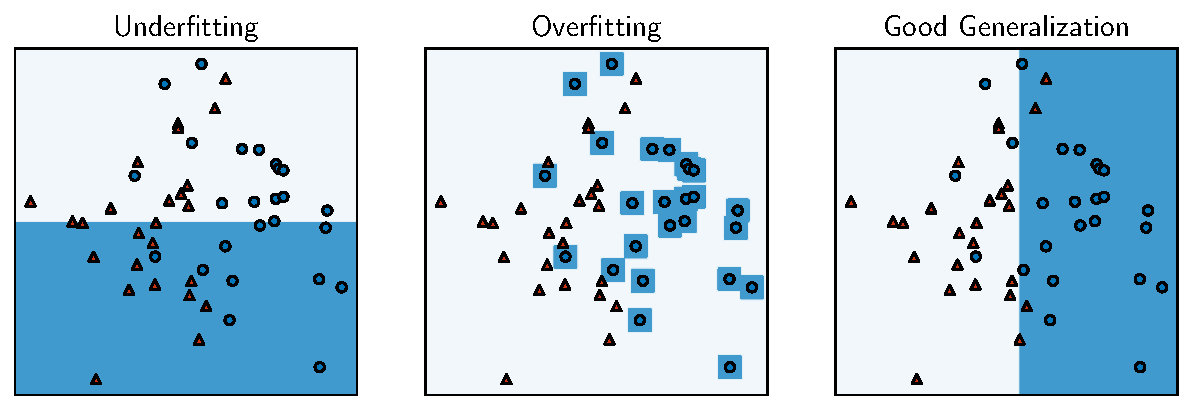
\includegraphics[width=1.0\textwidth]{chapter_1/figures/overfitting.pdf}
    \caption[Representation of the Underfitting, Overfitting and the Generalization]{
    Representation of the three situations (one per scatter plot) that can arise in statistical learning.
    The left figure corresponds to a hypothesis $\h$ that underfits the data: both the empirical risk $\Risk_{\dS}(\h)$ and the true risk $\Risk_{\D}(\h)$ are high.
    In the middle figure, the hypothesis $\h$ overfits the data: the empirical risk $\Risk_{\dS}(\h)=0$ but the true risk $\Risk_{\D}(\h)$ is high.
    The left figure represents the perfect case: the difference between the true risk $\Risk_{\D}(\h)$ and the empirical risk $\Risk_{\dS}(\h)$ is small as well as $\Risk_{\dS}(\h)$.
    }
    \label{chap:intro:fig:overfitting}
\end{figure}

\section{Generalization Bounds}
\label{chap:intro:sec:bound}
 
To upper-bound the generalization gap $\RiskLoss_{\D}(\h)-\RiskLoss_{\dS}(\h)$, we can provide a bound on the true risk $\RiskLoss_{\D}(\h)$ with high probability over the random choice of $\S\sim\D^\m$.
Such a bound is a {\it Probably Approximately Correct} (PAC) generalization bound~\citep{Valiant1984} and can be defined as follows.

\begin{definition}[PAC Generalization Bound] For any distribution $\D$ on $\X{\times}\Y$, for any data-dependent hypothesis set $\H=\{\h_{\S}\}_{\S\in(\X{\times}\Y)^\m}$ where $\h_{\S}$ is a hypothesis dependent on the learning sample $\S\in(\X{\times}\Y)^\m$, a PAC generalization bound is defined by
\begin{align*}
    \PP_{\S\sim\D^\m}\Big[ \RiskLoss_{\D}(\h_{\S}) \le \Phi \Big]\ge 1-\delta.
\end{align*}
\label{chap:intro:def:pac}
\end{definition}

{\it With high Probability} (with probability at least $1{-}\delta$), the true risk of the hypothesis $\h_{\S}$ is {\it Approximately Correct}, \ie, upper-bounded by $\Phi$.
Based on this definition, \citet{Valiant1984} has brought a computational framework: the PAC-Learnability.\footnote{\citeauthor{Valiant1984} won the Turing prize in 2010 for the definition of PAC-Learnability.}
A data-dependent hypothesis set $\H=\{\h_{\S}\}_{\S\in(\X{\times\Y})^\m}$ is PAC-Learnable if this high probability bound holds when the number of examples $m$ is polynomial in $1/\delta$ and $1/\Phi$.
In practice, to obtain such an upper bound $\Phi$, we make use of {\it concentration inequalities} (see \citet{BoucheronLugosiMassart2013} for an extensive introduction on the subject).
These inequalities allow us to bound an expectation (the true risk in our case) with its empirical counterpart (the empirical risk).
Depending on the concentration inequalities, one can obtain different frameworks, and so, different upper bounds $\Phi$.

\subsection{Uniform Convergence Bounds}
\label{chap:intro:sec:bound-uc}

The first framework introduced in the literature to obtain PAC generalization bounds is referred to as {\it uniform convergence} bounds~\citep{VapnikChervonenkis1968,VapnikChervonenkis1971}.
Given a hypothesis set $\H$ (not necessarily data-dependent), a uniform convergence bound holds for all hypotheses of $\H$.
By doing so, the true risk $\RiskLoss_{\D}(\h_{\S})$ of a data-dependent hypothesis $\h_{\S}\in\H$ is upper-bounded to obtain a PAC generalization bound.
This type of bounds takes the following form.

\begin{restatable}[Uniform Convergence Bound]{definition}{definitionUC}\label{chap:intro:def:uc} Let $\loss: \H \times(\X{\times}\Y)\rightarrow [0, 1]$ be a loss function and $\phi: [0,1]^2{\to}\Rbb$ a generalization gap.
A uniform convergence bound is defined such that if for any distribution $\D$ on $\X\times\Y$, for any hypothesis set $\H$, there exists a function $\PhiUC: (0,1]{\to} \Rbb$, such that for any  $\delta\in(0, 1]$ we have
\begin{align}
\PP_{\S\sim\D^{\m}}\LB\, \sup_{\h\in\H} \phi(\RiskLoss_{\D}(\h),\RiskLoss_{\dS}(\h)) \le \PhiUC\big(\delta\big) \RB\ge 1-\delta,\label{chap:intro:eq:uc}
\end{align}
where usually $\phi(\RiskLoss_{\D}(\h),\RiskLoss_{\dS}(\h))=\RiskLoss_{\D}(\h)-\RiskLoss_{\dS}(\h)$.
\end{restatable}

A uniform convergence bound consists in bounding the supremum of the generalization gap over the hypotheses $\h\in\H$ with the upper bound $\PhiUC\big(\delta\big)$ (with probability at least $1-\delta$ over the learning sample $\S\sim\D^\m$).
In other words, the inequality boils down to bound the generalization gap of all hypotheses $\h\in\H$ by an upper bound $\PhiUC\big(\delta\big)$ on the largest generalization gap; the hypothesis associated to the largest generalization gap is considered as the ``worst'' hypothesis in $\H$.
As we will see in the following, the upper bound $\PhiUC\big(\delta\big)$ depends also on the number of examples $\m$ in $\S$; we have simplified $\PhiUC\big(\delta\big)$ for readability.
Hence, if $\lim_{\m\rightarrow+\infty}\PhiUC(\delta)= 0$, with probability at least $1-\delta$ over $\S\sim\D^\m$, the empirical risk {\it converges uniformly} on $\H$ to the true risk $\RiskLoss_{\D}(\h)$.
Because of the uniform convergence, as we see in the two examples below, the upper bound $\PhiUC\big(\delta\big)$ depends on a {\it complexity} $\comp(\H)$ that measures, in some sense, the performance of the worst hypothesis in $\H$. 

\subsubsection{Uniform Convergence Bounds for Finite Hypothesis Sets}

The simplest complexity measure appearing in generalization bounds arises when considering a finite set $\H$ of hypotheses.
We recall an instantiation of uniform convergence bounds (\Cref{chap:intro:def:uc}) in the following theorem (see, \eg, \citet{MohriRostamizadehTalwalkar2012} for more details).

\begin{theorem}[Generalization Bound for Finite $\H$] For any distribution $\D$ on $\X{\times}\Y$, for any finite hypothesis set $\H$ ($\card(\H)<+\infty$), for any loss function $\loss: \H\times(\X{\times}\Y)\to [0,1]$, for any $\delta\in(0,1]$, we have 
\begin{align*}
    &\PP_{\S\sim\D^{\m}}\Bigg[\sup_{\h\in\H}\LB\RiskLoss_{\D}(\h)-\RiskLoss_{\dS}(\h)\RB \le  \underbrace{\sqrt{\frac{\ln\card(\H)+\ln\frac{1}{\delta}}{2\m}}}_{\PhiUC(\delta)}\,\Bigg] \ge 1{-}\delta,
\end{align*}
where $\card(\H)$ is the cardinal of the set $\H$.
Equivalently, with probability at least $1{-}\delta$ over $\S\sim\D^\m$, we have
\begin{align*}
    \forall \h\in\H,\quad \RiskLoss_{\D}(\h) \le \RiskLoss_{\dS}(\h)+ \sqrt{\frac{\ln\card(\H)+\ln\frac{1}{\delta}}{2\m}}.
\end{align*}
\label{chap:intro:theorem:finite}
\end{theorem}

In this case, the complexity measure for a finite hypothesis set is defined by $\comp(\H)=\card(\H)$.
According to this complexity measure, the more hypotheses in $\H$, the more complex the hypothesis set $\H$ is.
The computation of this complexity can be fast, making this generalization bound easy to evaluate and to obtain an upper bound on the generalization gap $\RiskLoss_{\D}(\h)-\RiskLoss_{\dS}(\h)$.
However, the bound does not converges when the cardinality of the set is large, \eg, when $\card(\H)\ge e^\m$ for $\m\in\Nbb$, the upper bound of \Cref{chap:intro:theorem:finite} is  $ \sqrt{\tfrac{1}{2}} \le \sqrt{\tfrac{1}{2\m}(\ln\card(\H)+\ln\frac{1}{\delta})}$.
Hence, there is a need to develop generalization bounds for hypothesis sets $\H$ with large $\card(\H)$ or infinite hypothesis sets.
Indeed, these types of set are usually considered in practice, \eg, the set of linear classifiers.

\subsubsection{VC-Dimension-based Generalization Bounds}

When the loss is the 01-loss, a bound for infinite hypothesis sets is proposed based on a complexity measure $\comp()$ called the {\sc Vapnik}-{\sc Chervonenkis} (VC)-Dimension \citep{VapnikChervonenkis1968,VapnikChervonenkis1971}.

\begin{definition}[{\sc Vapnik}-{\sc Chervonenkis} (VC) Dimension]\label{chap:intro:def:vc-dim} Given a hypothesis set $\H$ with hypotheses $h:\X\to\{-1, +1\}$ (for binary classification), the VC-dimension of the set $\H$ is defined as
\begin{align*}
    \vc(\H) \defeq \max\LC \m \;:\; \forall \S\in(\X{\times}\Y)^\m, \exists \h\in\H \ \text{\st}\ \Risk_{\dS}(\h) = 0 \RC,
\end{align*}
where $\Risk_{\dS}(\h)=\frac{1}{\m}\sum_{i=1}^{\m}\indic[\h(\x)\ne \y]$.
\end{definition}
Put into words, the VC-Dimension $\comp(\H)=\vc(\H)$ of a hypothesis set $\H$ is the maximum number of examples that a hypothesis $\h$ from $\H$ can perfectly fit in binary classification.
Note that if the hypothesis set $\H$ is infinite, its associated VC-dimension $\vc(\H)$ can be finite.
For example, the VC-Dimension of the $\d$-dimensional linear classifiers is $\d+1$ (see \citet[Example~3.12]{MohriRostamizadehTalwalkar2012} for a proof) even if the set of linear classifiers $\H$ is infinite; we illustrate in \Cref{chap:intro:fig:vc_dim} the $2$-dimensional case.
Thanks to this complexity measure, we can prove the following generalization bound \citep[Theorem~3.17, Corollaries 3.18 and 3.19]{MohriRostamizadehTalwalkar2012}.

\begin{figure}
    \centering
    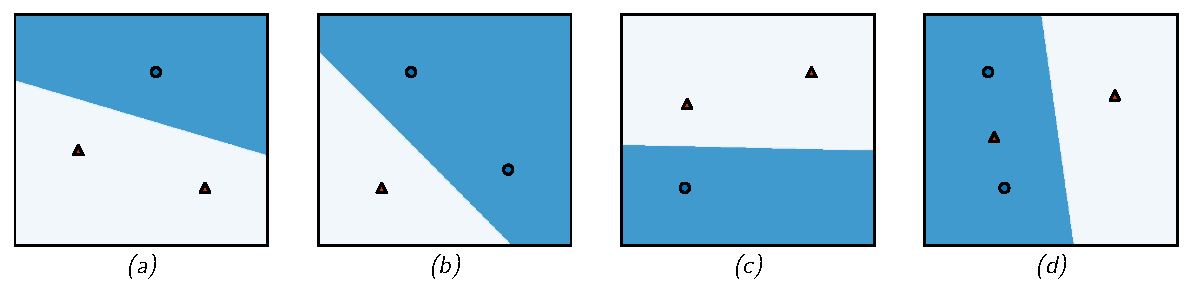
\includegraphics[width=\textwidth]{chapter_1/figures/vc_dim.pdf}
    \caption[Illustration of the VC-dimension for Linear Classifiers in $2$-dimension]{
    Illustration of the VC-dimension for linear classifiers in $2$-dimension. 
    When $\m{=}3$, a linear classifier can always perfectly fit the data, \ie, $\Risk_{\dS}(\h)=0$ (as shown in the plot {\it (a)}, {\it (b)}, and {\it (c)}).
    However, when $\m{=}4$, the empirical risk $\Risk_{\dS}(\h)\ge 0$ for all linear classifiers (as illustrated in the plot {\it (d)}). 
    Hence, in this case, the VC-Dimension is $\vc(\H)=3$.
    }
    \label{chap:intro:fig:vc_dim}
\end{figure}

\begin{theorem}[VC-Dimension-based Generalization Bounds]\label{chap:intro:theorem:vc-dim} For any distribution $\D$ on $\X{\times}\Y$, for any set $\H$ with hypotheses $h:\X\to\{-1, +1\}$ and VC-Dimension $\vc(\H)$, for any $\delta\in(0,1]$, we have 
\begin{align*}
    &\PP_{\S\sim\D^{\m}}\Bigg[\sup_{\h\in\H}\LB\Risk_{\D}(\h)-\Risk_{\dS}(\h)\RB \le  \underbrace{\sqrt{\frac{2\vc(\H)\LP1+\ln\frac{\m}{\vc(\H)}\RP}{\m}} + \sqrt{\frac{\ln\frac{1}{\delta}}{2\m}}}_{\PhiUC(\delta)}\,\Bigg] \ge 1{-}\delta.
\end{align*}
Equivalently, with probability at least $1{-}\delta$ over $\S\sim\D^\m$, we have
\begin{align*}
    \forall \h\in\H,\quad \Risk_{\D}(\h) \le \Risk_{\dS}(\h)+ \sqrt{\frac{2\vc(\H)\LP1+\ln\frac{\m}{\vc(\H)}\RP}{\m}} + \sqrt{\frac{\ln\frac{1}{\delta}}{2\m}}.
\end{align*}
\end{theorem}

Hence, if we know the VC-dimension of the hypothesis set $\H$ of interest, the bound becomes easily computable to obtain an upper bound of the generalization gap.  
Furthermore, it is possible to prove that the ERM algorithm is consistent~\citep{Vapnik1998} thanks to this bound \citep[see Proposition 4.1][]{MohriRostamizadehTalwalkar2012}.
When ERM is consistent, {\it (a)} the empirical risk $\Risk_{\dS}(\h)$ of the classifier $\h$ obtained by ERM converges in probability to $\inf_{\h'\in\H}\Risk_{\D}(\h')$, and {\it (b)} its true risk $\Risk_{\dS}(\h)$ converges in probability to $\inf_{\h'\in\H}\Risk_{\D}(\h')$ as well.
Nevertheless, one drawback of the VC-Dimension is that it is only for binary classifiers and the 01-loss;
there are several extensions for the multi-class setting, we introduce one of them: the Rademacher complexity~\citep{BartlettMendelson2002}.

\subsubsection{Rademacher-complexity-based Generalization Bounds}

The Rademacher complexity~\citep{BartlettMendelson2002} of a hypothesis set $\H$ can be defined as follows.

\begin{definition}[Rademacher Complexity]\label{chap:intro:def:rademacher}
Given a hypothesis set $\H$ and a loss function $\loss: \H\times(\X{\times}\Y) \to [0, 1]$, the Rademacher complexity $\rad(\H)$ of the set $\H$ is defined as 
\begin{align*}
    \rad(\H) &= \EE_{\S\sim\D^\m}\EE_{\{\kappa_1,\dots, \kappa_\m\}\sim\kappacal^\m}\sup_{\h\in\H} \frac{1}{\m}\sum_{i=1}^{\m}\kappa_i\loss(\h, (\x_i, \y_i)),\\
    &\text{where $\kappacal$ is the Rademacher distribution, \ie, }\kappacal(+1) = \kappacal(-1) = \frac{1}{2}.
\end{align*}
\end{definition}

Given a learning sample $\S\sim\D^\m$ and the Rademacher variables $\{\kappa_1,\dots, \kappa_\m\}\sim\kappacal^\m$, the supremum is attained when the loss $\loss(\h, (\x_i, \y_i))$ is maximized (\resp minimized) when $\kappa_i{=}+1$ (\resp $\kappa_i{=}-1$).
Then, the Rademacher complexity is the expected supremum over the learning sample and the Rademacher variables.
For example, in binary classification, the Rademacher complexity measures the capacity of the hypotheses in $\H$ to learn examples with random labels.
As illustrated in \Cref{chap:intro:fig:rademacher} when $\m=3$, (multi-class) linear classifiers are able to fit any data points with random labels.
In this case, the Rademacher complexity $\rad(\H)=1$, but hopefully when $m\rightarrow+\infty$ the Rademacher complexity of the linear classifiers tends to $0$ at a rate of $O\big(\sqrt{\tfrac{1}{m}}\big)$ (see, \eg, \citet{KakadeSridharanTewari2008}, for the binary classification case).

\begin{figure}
    \centering
    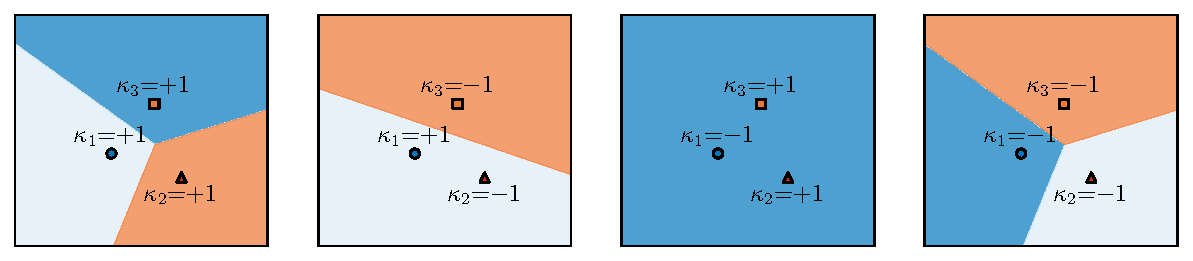
\includegraphics[width=\textwidth]{chapter_1/figures/rademacher.pdf}
    \caption[Illustration of the Rademacher Complexity in Multi-class Classification]{
    Illustration of the Rademacher complexity $\rad(\H)$ in multi-class classification with $\loss(\h, (\x, \y)) = \indic[\h(\x)\ne \y]$ and $\m=3$.
    Given a learning sample $\S\in(\X\times\Y)^2$, we show for each $(\kappa_1, \kappa_2)\in\{-1, +1\}^2$ the examples and a classifier $\h$ \st $\RiskLoss_{\Scal}(\h)=\sup_{\h\in\H} \frac{1}{\m}\sum_{i=1}^{\m}\kappa_i\loss(\h, (\x_i, \y_i))$.
    }
    \label{chap:intro:fig:rademacher}
\end{figure}

From McDiarmid's concentration inequality~\citep{McDiarmid1989}, \citet{BartlettMendelson2002} derived the following generalization bound that depends on the Rademacher complexity.

\begin{theorem}[Rademacher-complexity-based Generalization Bound]\label{chap:intro:theorem:rademacher}
For any distribution $\D$ on $\X\times\Y$, for any hypothesis set $\H$, for any loss function $\loss: \H\times(\X{\times}\Y) \to [0, 1]$, for any $\delta\in(0,1]$, we have
\begin{align*}
    &\PP_{\S\sim\D^{\m}}\Bigg[\sup_{\h\in\H}\LB\RiskLoss_{\D}(\h)-\RiskLoss_{\dS}(\h)\RB \le  \underbrace{2\rad(\H) + \sqrt{\frac{\ln\frac{1}{\delta}}{2\m}}}_{\PhiUC(\delta)}\,\Bigg]\ge 1{-}\delta.
\end{align*}
Equivalently, with probability at least $1{-}\delta$ over $\S\sim\D^\m$, we have
\begin{align*}
    \forall \h\in\H,\quad \RiskLoss_{\D}(\h) \le \RiskLoss_{\dS}(\h)+ 2\rad(\H) + \sqrt{\frac{\ln\frac{1}{\delta}}{2\m}}.
\end{align*}
\end{theorem}

Put into words, the generalization gap is upper-bounded by the Rademacher complexity of the set $\H$ along with a tight term when the number of examples $\m$ is large.
As for the VC-Dimension-based bound, if we have an analytic expression of the complexity (or an upper bound), we can compute the generalization bound for all hypotheses $\h$ in $\H$.
Since the bound holds for all $\h\in\H$ (due to $\sup_{\h\in\H}$), it can be seen as a {\it worst-case} analysis.
Indeed, the same upper bound (\ie, $\PhiUC(\delta)$) holds for all $\h\in\H$, including the best, but also the worst (with the largest generalization gap $\RiskLoss_{\D}(\h){-}\RiskLoss_{\dS}(\h)$).
This {\it worst-case} analysis makes the derivation of non-vacuous bounds hard (\ie, with $\PhiUC(\delta){<}1$).
Hence, other generalization bounds have been developed to avoid this worst-case analysis as we see in the next section. 

\subsection{Algorithmic-dependent Generalization Bounds}
\label{chap:intro:sec:bound-algo}

Let consider an algorithm that takes a learning sample $\S\in(\X\times\Y)^\m$ as input and outputs the hypothesis $\h_{\S}$ belonging to the hypothesis set $\H=\{\h_{\S}\}_{\S\in(\X{\times}\Y)^\m}$.
Thanks to this algorithm, one can derive generalization bounds for the hypothesis $\h_\S$ given $\S\sim\D^\m$ that has the following form.

\begin{restatable}[Algorithmic-dependent Generalization Bound]{definition}{definitionALGODEP}\label{chap:intro:def:algo} Let $\loss: \H \times(\X{\times}\Y)\rightarrow [0, 1]$ be a loss function and $\phi: [0,1]^2{\to}\Rbb$ a generalization gap. 
An algorithmic-dependent generalization bound is defined such that if for any distribution $\D$ on $\X\times\Y$, there exists a function $\PhiA: (0,1]{\to} \Rbb$, such that for any  $\delta\in(0, 1]$ we have
\begin{align}
    \PP_{\S\sim\D^m}\Big[ \phi(\RiskLoss_{\D}(\h_{\S}), \RiskLoss_{\dS}(\h_{\S})) \le \PhiA(\delta) \Big] \ge 1{-}\delta,\label{chap:intro:eq:algo}
\end{align}
where usually $\phi(\RiskLoss_{\D}(\h), \RiskLoss_{\dS}(\h)) = \RiskLoss_{\D}(\h) - \RiskLoss_{\dS}(\h)$ and $\h_{\S}$ is the hypothesis learned from an algorithm with $\S\sim\D^\m$.

\end{restatable}

\looseness=-1
According to \Cref{chap:intro:def:algo}, one can derive an upper bound $\PhiA(\delta)$ of the generalization gap $\RiskLoss_{\D}(\h_{\S})-\RiskLoss_{\dS}(\h_{\S})$ for the algorithmic-dependent hypothesis $\h_{\S}$.
Actually, to derive such an upper bound $\PhiA(\delta)$, a property of the considered learning algorithm must be considered; we recall in the following the algorithmic stability~\citep{BousquetElisseeff2002} and the algorithmic robustness of~\citet{XuMannor2010,XuMannor2012}.

\subsubsection{Stability-based Generalization Bounds}

The first algorithmic property we recall is the uniform stability~\citep{BousquetElisseeff2002} and is defined as follows.

\begin{definition}[Uniform Stability]\label{chap:intro:def:stability} Given the hypothesis set $\H=\{\h_{\S}\}_{\S\in(\X\times\Y)^\m}$ and a loss function $\loss:\H\times(\X\times\Y)\to [0,1]$, an algorithm is $\stab$-uniformly stable if
\begin{align*}
    \sup_{\substack{\S,\S' \in (\X\times\Y)^\m\\\text{s.t.}\  \Delta(\S,\S')=1}}\sup_{(\x,\y)\in\X{\times}\Y} \Big\vert \loss(h_{\S}, (\x,\y))-\loss(h_{\S'}, (\x,\y)) \Big\vert \le \stab,
\end{align*}
where $\Delta(\S, \S')=\sum_{i=1}^\m\indic\LB (\x_i,\y_i) \ne (\x_i',\y_i') \RB$ is the Hamming distance between the learning samples $\S$ and $\S'$.
\end{definition}

For two learning samples $\S$ and $\S'$ that differ from only one example (\ie, that are very similar), the uniform stability $\stab$ measures how much stable the algorithm is under small changes in the learning sample.
To be stable, the difference of losses between the hypotheses $\h_{\S}$ and $\h_{\S'}$ must be small (and upper bounded by $\stab$) for all examples $(\x,\y)\in\X\times\Y$.
Typically, $\stab$ can be seen as a complexity measure that depends on the number of examples $\m$. 
When $\stab=O(\frac{1}{\sqrt{\m}})$ or $\stab=O(\frac{1}{\m})$, the algorithm becomes more stable as the number of examples in $\S$ increases.
The notion of algorithmic stability is illustrated and summarized in \Cref{chap:intro:fig:stability}.
\begin{figure}
    \centering
    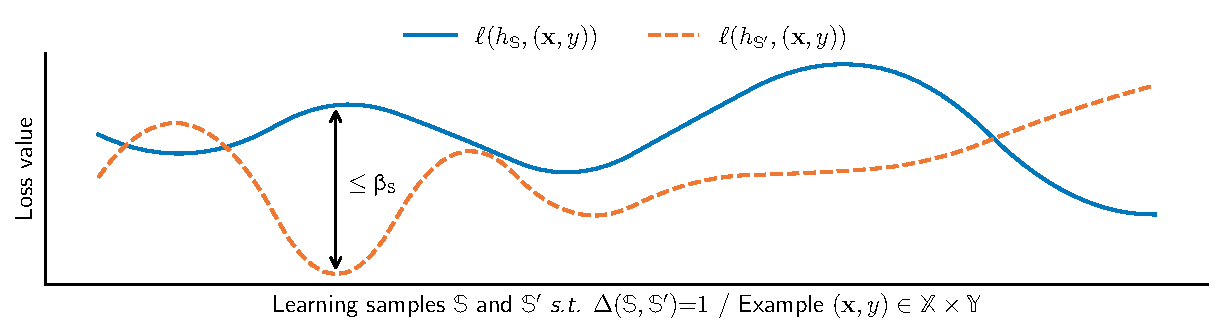
\includegraphics[width=\textwidth]{chapter_1/figures/stability.pdf}
    \caption[Schematic Representation of the Uniform Stability]{
    Schematic representation of the notion of stability $\stab$.
    The two curves represents the losses $\loss(\h_\S, (\x,\y))$ and $\loss(\h_{\S'}, (\x,\y))$ (the y-axis) for different combinations of examples $(\x, \y)\in \X{\times}\Y$ and learning samples $\S$ and $\S'$ that differs from one example (the x-axis).
    }
    \label{chap:intro:fig:stability}
\end{figure}
From this notion of uniform stability and McDiarmid's inequality~\citep{McDiarmid1989}, the following generalization bounds can be derived~\citep{BousquetElisseeff2002}.

\begin{theorem}[Stability-based Bounds] Given the hypothesis set $\H = \{\h_{\S}\}_{\S\in(\X{\times}\Y)^\m}$, for any distribution $\D$ on $\X\times\Y$, for any loss function $\loss: \H\times(\X\times\Y) \to [0,1]$, for any $\stab$-uniformly stable algorithm, for any $\delta\in(0,1]$, we have 
\begin{align*}
    \PP_{\S\sim\D^\m}\LB\RiskLoss_{\D}(\h_{\S})-\RiskLoss_{\dS}(\h_{\S}) \le 2\stab + (4\m\stab{+}1)\sqrt{\frac{\ln\frac{1}{\delta}}{2\m}}\,\RB\ge 1{-}\delta.
\end{align*}
Equivalently, with probability at least $1{-}\delta$ over $\S\sim\D^\m$, we have
\begin{align*}
    \RiskLoss_{\D}(\h_{\S}) \le \RiskLoss_{\dS}(\h_{\S}) + 2\stab + (4\m\stab{+}1)\sqrt{\frac{\ln\frac{1}{\delta}}{2\m}}.
\end{align*}
\end{theorem}

Note that, for this particular bound, if the algorithm is $O(1)$-uniformly stable, the above bound does not converge and is vacuous.
In contrast, an $O(\frac{1}{\sqrt{\m}})$-uniformly stable algorithm gives an $O(\frac{1}{\sqrt{\m}})$ convergence rate.
Recently, tighter generalization bounds have been improved: the bound converges with a $O(\frac{1}{\m})$-uniformly stable algorithm \citep{FeldmanVondrak2018,FeldmanVondrak2019,BousquetKlochkovZhivotovskiy2020}.
As for the uniform-convergence-based bounds, an analytical expression of the stability $\stab$ has to be derived to compute the bound.

\subsubsection{Robustness-based Generalization Bounds}

Another learning algorithm property used to derive generalization bounds is the algorithmic robustness.
This notion can be defined as follows.

\begin{definition}[Robustness]\label{chap:intro:def:robustness} Given the hypothesis set $\H=\{\h_{\S}\}_{\S\in(\X\times\Y)^\m}$, a loss function $\loss:\H\times(\X\times\Y)\to [0,1]$ and $N$ disjoint sets \st $(\X{\times}\Y)=\bigcup_{i=1}^{N}\Z_i$, the algorithm is $(\{\Z_i\}_{i=1}^N, \rob)$-robust\protect\footnotemark\ if
\begin{align*}
    \sup_{\S\in(\X{\times}\Y)^\m}\sup_{i\in\{1,\dots,N\}}\sup_{(\x,\y),(\x',\y')\in\Z_i}\Big\vert \loss(\h_\S, (\x, \y)) - \loss(\h_\S, (\x', \y'))\Big\vert \le \rob.
\end{align*}
\end{definition}
\footnotetext{In the original definition, the robust parameter $\rob$ can depend on the learning sample $\S\sim\D^\m$. 
However, in the examples of \citet{XuMannor2012} for the classification setting, $\rob$ depends only on the number of examples $\m$.}

\begin{figure}
    \centering
    \includestandalone[width=1.0\textwidth]{chapter_1/figures/robustness}
    \caption[Schematic Representation of the Algorithmic Robustness]{
    Schematic representation of the notion of algorithmic robustness. 
    On the left plot, an example of partition $\{\Z_i\}_{i=1}^{N}$ for the set $\X\times\Y$ is shown.
    Then, for a given subset $\Z_i$, we represent on the right plot the losses $\loss(\h_\S, (\x,\y))$ and $\loss(\h_\S, (\x', \y'))$ for any learning sample $\S$, and examples $(\x,\y)\in\Z_i$ and $(\x',\y')\in\Z_i$.
    }
    \label{chap:intro:fig:robustness}
\end{figure}
For each subset $\Z_i\subseteq \X{\times}\Y$, the difference of losses between two examples $(\x,\y)\in\Z_i$ and $(\x',\y')\in\Z_i$ has to be upper-bounded by $\rob$;
for pedagogical purposes, we summarize in \Cref{chap:intro:fig:robustness} the algorithmic robustness.
The following bound can be derived based on this property and thanks to the Breteganolle-Huber-Carol concentration inequality \citep[Proposition A.6.6]{VaartWellner1996}.

\begin{theorem}[Robustness-based Bounds]
\looseness=-1
Given the hypothesis set $\H = \{\h_{\S}\}_{\S\in(\X{\times}\Y)^\m}$, for any distribution $\D$ on $\X\times\Y$, for any loss function $\loss: \H\times(\X\times\Y) \to [0,1]$, for any $(\{\Z_i\}_{i=1}^N, \rob)$-robust algorithm, for any $\delta\in(0,1]$, we have 
\begin{align*}
    \PP_{\S\sim\D^\m}\LB\RiskLoss_{\D}(\h_\S) \le \RiskLoss_{\S}(\h_\S) + \rob + \sqrt{\frac{2N\ln2+ 2\ln\frac{1}{\delta}}{2\m}}\RB\ge 1-\delta.
\end{align*}
Equivalently, with probability at least $1-\delta$ over $\S\sim\D^\m$, we have
\begin{align*}
\RiskLoss_{\D}(\h_\S) \le \RiskLoss_{\S}(\h_\S) + \rob + \sqrt{\frac{2N\ln2+ 2\ln\frac{1}{\delta}}{2\m}}.
\end{align*}
\end{theorem}

The bound is computable if we have an analytical expression of the algorithmic robustness parameter $\rob$.
Ideally, the robustness parameter $\rob$ must depend on $\m$ for the bound to converge.
Furthermore, we can remark that there is a trade-off to find between the number of disjoint subsets $N$ and the robust upper bound $\rob$.  
Indeed, the larger $N$ is, the smaller we expect the parameter $\rob$ to be.
However, if $N \ge \m$, the bound cannot be tighter than $\sqrt{\ln(2)}$, and hence, does not converge towards $0$ when $\m\rightarrow+\infty$.\\

The major drawback of the algorithmic-based bounds is that we have to derive the parameter $\stab$ or $\rob$ for each algorithm.
Hence, such derivation can be tedious, and the upper-bound $\PhiA(\delta)$ is constant over the learning sample $\S\sim\D^\m$.
Another kind of bounds -- called {\it PAC-Bayesian Bounds} -- does not have such drawbacks and is appealing because of its facility to derive learning algorithms from it, as we will see in \Cref{part:contrib-pac-bayes}.  
An in-depth introduction of these bounds is done in \Cref{chap:pac-bayes}, but we give a quick overview in the rest of the chapter.

\subsection{PAC-Bayesian Generalization Bounds}

PAC-Bayesian bounds were introduced notably by \citet{ShaweTaylorWilliamson1997,McAllester1999}, but it has been improved since then \citep{Seeger2002,Maurer2004,Catoni2007}.
The PAC-Bayesian bounds differ significantly from the ones of \Cref{chap:intro:sec:bound-uc,chap:intro:sec:bound-algo}: they require a probability distribution (denoted by $\Q$) on the hypothesis set $\H$.
This distribution is used to assign a weight $\Q(\h)$ to each hypothesis $\h\in\H$. 
Hopefully, when the hypothesis $\h$ generalizes well, its weight $\Q(\h)$ should be high.
Thanks to this assumption, we can consider a {\it stochastic} hypothesis: given an input $\x\in\X$, its output is obtained by {\it (1)} sampling a hypothesis $\h$ from $\Q$, and by {\it (2)} computing the prediction $\h(\x)$.
Actually, the PAC-Bayesian bounds allow us to upper-bound the true risk of {\it stochastic} hypotheses which is the {\it expected} true risk of a hypothesis sampled from a distribution $\Q$.
More precisely, the PAC-Bayesian bounds study the {\it expected} generalization gap $\EE_{\h\sim\Q}\RiskLoss_{\D}(\h)-\EE_{\h\sim\Q}\RiskLoss_{\dS}(\h)$.
We present one bound derived by \citet{Maurer2004} in the following theorem.

\begin{theorem}[PAC-Bayesian Bound of \citet{Maurer2004}]
For any distribution $\D$ over $\X\times\Y$, for any hypothesis set $\H$, for any loss function $\loss: \H\times (\X\times\Y) \rightarrow [0, 1]$, for any distribution $\P$ on $\H$ (defined \apriori), for any $\delta\in(0,1]$, we have
\begin{align*}
\PP_{\S\sim\D^\m}\LB
\begin{array}{l}
    \text{For all distributions } \Q \text{ on } \H,\\
    \EE_{h\sim\Q} \RiskLoss_{\D}(\h) \le \EE_{h\sim\Q}\RiskLoss_{\dS}(\h) + \sqrt{\frac{1}{2\m}\LB \KL(\Q\|\P) + \ln\frac{2\sqrt{\m}}{\delta}\RB}
\end{array}
\RB \ge 1-\delta,
\end{align*}
where the Kullback–Leibler (KL) divergence is defined as $\KL(\Q\|\P)=\EE_{\h\sim\Q}\ln\frac{\Q(\h)}{\P(\h)}$.
Equivalently, with probability at least $1-\delta$ over $\S\sim\D^\m$, we have
\begin{align*}
\forall\text{ distributions } \Q \text{ on } \H,\quad \EE_{h\sim\Q}\RiskLoss_{\D}(\h) \le \EE_{h\sim\Q}\RiskLoss_{\dS}(\h) + \sqrt{\frac{1}{2\m}\LB \KL(\Q\|\P) + \ln\frac{2\sqrt{\m}}{\delta}\RB}.
\end{align*}
\label{chap:intro:theorem:maurer}
\end{theorem}

The bound of this theorem depends on the KL divergence between $\Q$ and $\P$, which measures the complexity of the hypothesis sampled from $\Q$.
Indeed, given a distribution $\P$ selected \apriori before having the learning sample $\S\sim\D^\m$, the higher $\KL(\Q\|\P)$, the more different the two distributions $\Q$ and $\P$ are.
Hence, in some sense, the KL divergence captures how much the distribution $\Q$ depends on the data $\S$.

\section{Conclusion and Summary}

In this chapter, we have seen an introduction to statistical learning.
It includes an overview of algorithms to perform hypothesis selection: Empirical Risk Minimization and Structural Risk Minimization.
Additionally, we recall some generalization bounds based on the uniform convergence (\eg, with the VC-Dimension or the Rademacher complexity) or an algorithmic property (\eg, the stability or the robustness)
Moreover, we recall a generalization bound from a key theory in our contributions: the PAC-Bayesian theory.
This is why we recall, with more details, in the next chapter the PAC-Bayesian theory.